% Отключаем subsection!
\PassOptionsToPackage{subsection=false}{beamerouterthememiniframes}
\documentclass[usenames,dvipsnames,pdftex,unicode,hidelinks]{beamer}
  \usepackage{cmap}
  \usepackage[T2A]{fontenc}
  \usepackage[utf8]{inputenc}
  \usepackage[english,russian]{babel}
  \usepackage{wasysym}
  \usepackage{gensymb} % для \degree
  \usepackage{mathtext} % для кириллицы в формулах
    \DeclareSymbolFont{T2Aletters}{T2A}{cmr}{m}{it} % кириллица в формулах курсивом
  \usepackage{tikz}
    \usetikzlibrary{positioning,fit,backgrounds}
    \graphicspath{{../img/}{../../img/}}
  \usepackage{numprint}
    % алиас и настройки для numprint
    \newcommand{\num}[1]{\numprint{#1}}
    \npthousandsep{\,}
    \npthousandthpartsep{}
    \npdecimalsign{,}
  \usepackage{array} % для \arraybackslash в таблице

  % add frame number to footline
  \let\oldmacro\insertshorttitle
  \renewcommand*\insertshorttitle{
    \oldmacro\hfill
    -\,\insertframenumber\,- % TODO: temporary comment total count % \,/\,\inserttotalframenumber
  }
  % TODO HACK: вместо института выводим автора
  \renewcommand*\insertshortinstitute{
    \insertshortauthor
  }

  % hide navigation symbols
  \beamertemplatenavigationsymbolsempty

  \usetheme{Szeged}%{Warsaw}
  \usecolortheme{crane}
  \usefonttheme{structurebold}
  \useinnertheme{rounded}
  % Патчим некоторые цвета
  %\setbeamertemplate{background canvas}[vertical shading][bottom=black!60!blue,top=black!80!blue]
  \setbeamercolor{block title}{bg=title.bg}
  \setbeamercolor{block body}{bg=title.bg!60}

  \setbeamercovered{transparent}

  \newcommand{\muted}[1]{\textcolor{gray}{#1}}

  % Начало раздела с показом его заголовка на весь кадр
  \newcommand{\splashsection}[1]{
    \section{} % чтобы этот слайд не относился
    {
      \setbeamercolor{background canvas}{bg=Goldenrod!50!Dandelion!50}
      \begin{frame}[plain]
        \begin{center}
          \huge \textbf{#1}
        \end{center}
      \end{frame}
    }
    \section{#1}
    \subsection{#1} % NB: оно не будет отображаться, т.к. subsection'ы отключены
  }

  \newcommand{\operation}[2]{
    \begin{enumerate}
        \setcounter{enumi}{#1}
      \item #2
    \end{enumerate}
  }

  \newcommand{\vect}[1]{\vec{#1}} % единое выделение векторов (стрелкой)
  \newcommand{\matx}[1]{\mathbf{#1}} % единое выделение матриц (полужирным)
  \newcommand{\transposed}{\top} % единый знак транспонирования (U+22A4 down tack)
  \newcommand{\conj}[1]{#1^*} % единое обозначение комплексного сопряжения (черта сверху)
  \renewcommand{\le}{\leqslant} % <= с наклонной нижней перекладиной
  \renewcommand{\ge}{\geqslant} % >= с наклонной нижней перекладиной
  \renewcommand{\phi}{\varphi} % phi завитушкой

  \newcommand{\todo}[1]{\textbf{\textcolor{red}{TODO: #1}}}

\title{Рецепт пивного печенья}
\author[Л. Ф. Чайковская]{%
  \texorpdfstring{Автор~--- Л.\,Ф.\,Чайковская\\
    \muted{ \small преподаватель кафедры дифференциальных~уравнений, куратор
    группы 214 ММФ~НГУ (1982--1987 годов обучения) }
  }{Л. Ф. Чайковская}
}

\institute{\muted{broght to you by \textit{NIA} \& Mama}}

\date{ 4 ноября 2013 г. }

\begin{document}

  % Local background must be enclosed by curly braces for grouping.
  {
    \usebackgroundtemplate{
      % TODO BG?
    }
    \begin{frame}[plain]
      \titlepage
    \end{frame}
  }

  \splashsection{Продукты}
  
  \begin{frame}{Что купить}
    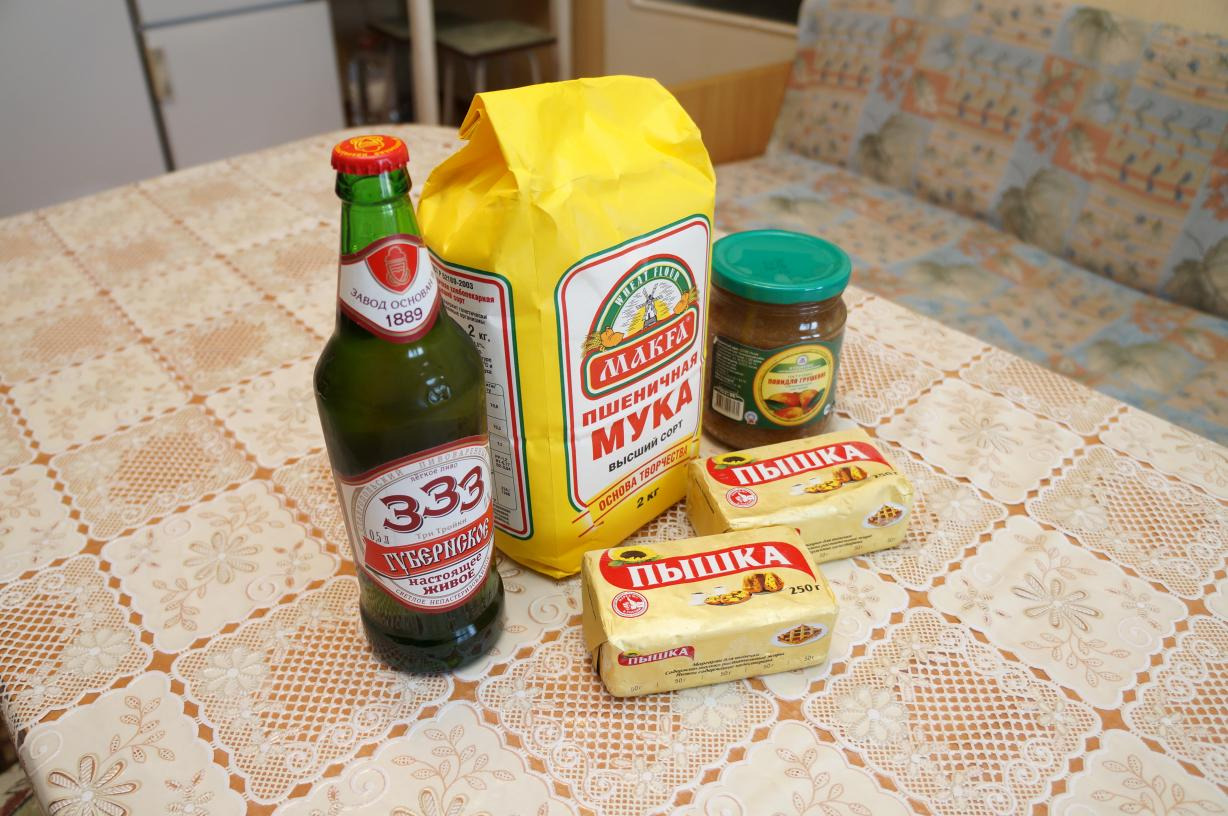
\includegraphics[width=\textwidth]{products}
  \end{frame}

  \begin{frame}{Пропорции}
    \begin{center}
      \def\arraystretch{1.5}%  1 is the default, change whatever you need WARNING: GLOBAL!
      % Centered columns with width: http://tex.stackexchange.com/a/5018/24732
      \begin{tabular}{|>{\centering\arraybackslash}p{4.5cm}|>{\centering\arraybackslash}p{4.5cm}|}
        \hline
        \textbf{1 порция} & \textbf{2 порции} \\
        (1,5--2 противня) & (3--4 противня) \\
        \hline\hline
        1 стакан пива\footnote{лучше непастеризованное} & 1 бутылка (0,5\,л) пива \\
        250\,г маргарина\footnote{лучше <<Пышка>>} & 500\,г маргарина \\
        $\approx 3$ стакана муки & $\approx 6$ стаканов муки \\
        \hline
        \multicolumn{2}{|c|}{+ повидло средней густоты\footnote{чтобы хорошо размазывалось, но не текло}} \\
        \hline
      \end{tabular}
    \end{center}
  \end{frame}

  \begin{frame}{Задание со звёздочкой}
    \uncover<+->{
      \begin{block}{Бонус}
        С посыпкой маком эти печеньки \alert{вкуснее}
      \end{block}
    }
    \uncover<+->{
      \begin{block}{Проблема}
        На данный момент купить кондитерский мак в Краснодаре
        из-за ограничений ГосНаркоКонтроля \alert{нельзя}
      \end{block}
    }
    \uncover<+->{
      \begin{block}{Постановка задачи}
        Разобраться, в чём реально состоят запреты, и выяснить,
        \alert{как купить мак} для благих целей \muted{(пекарни же где-то его берут)}
      \end{block}
    }
  \end{frame}
  
  \splashsection{Тесто}

  \begin{frame}{Растопить маргарин}
    \begin{center}
      % TODO use counter. Caveat: repetition on slides :(
      \operation{0}{Маргарин растопить на медленном огне, \alert{чтобы не закипел}}

      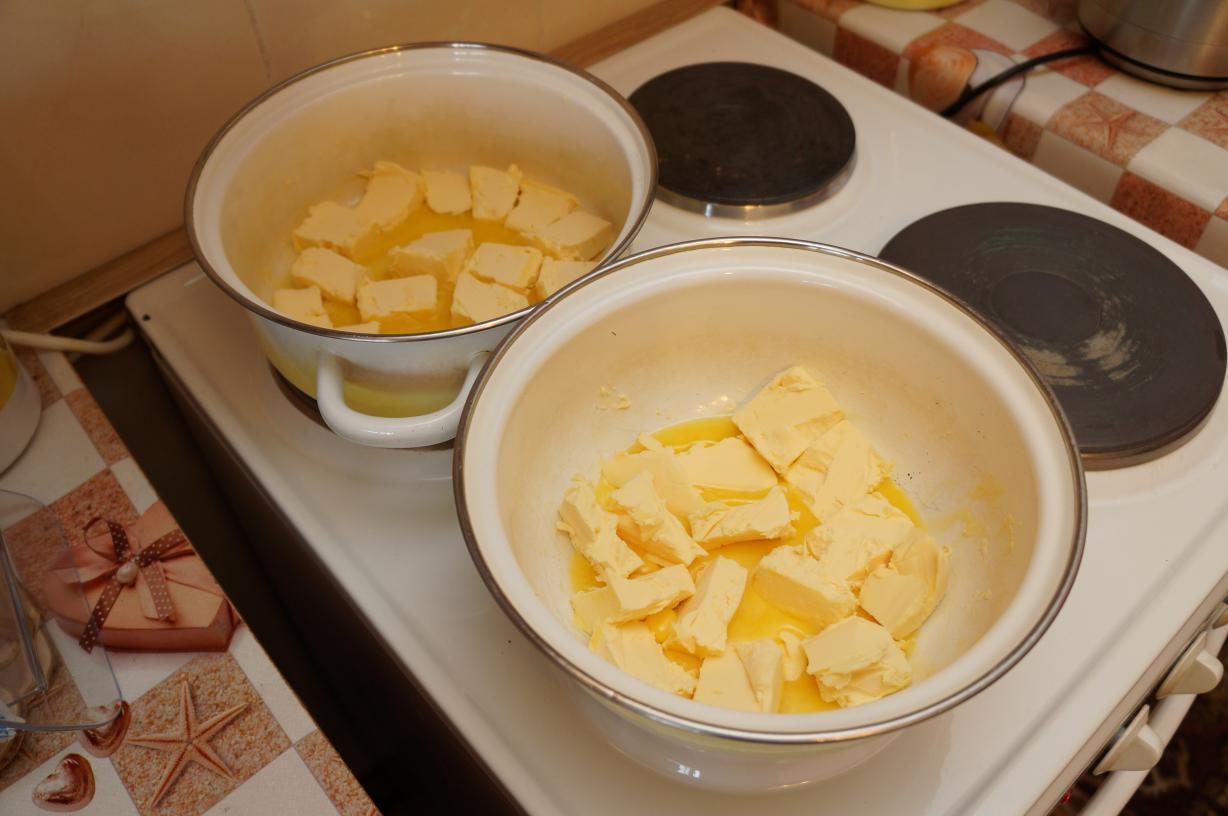
\includegraphics[height=0.7\textheight]{margarine-0}
    \end{center}
  \end{frame}

  \begin{frame}{Влить пиво}
    \begin{center}
      \operation{1}{Влить в растопленный маргарин пиво}

      \foreach \n in {1, 2} {
        \only<\n>{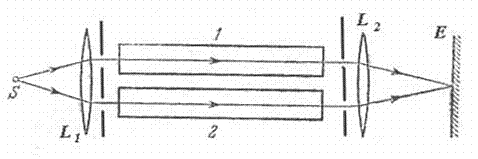
\includegraphics[height=0.7\textheight]{margarine-\n}}
      }
    \end{center}
  \end{frame}

  \begin{frame}{Добавить муку}
    \begin{center}
      \operation{2}{Добавить просеянную муку, вымесить тесто чуть гуще,\\
        чем обычное дрожжевое тесто для пирожков}

      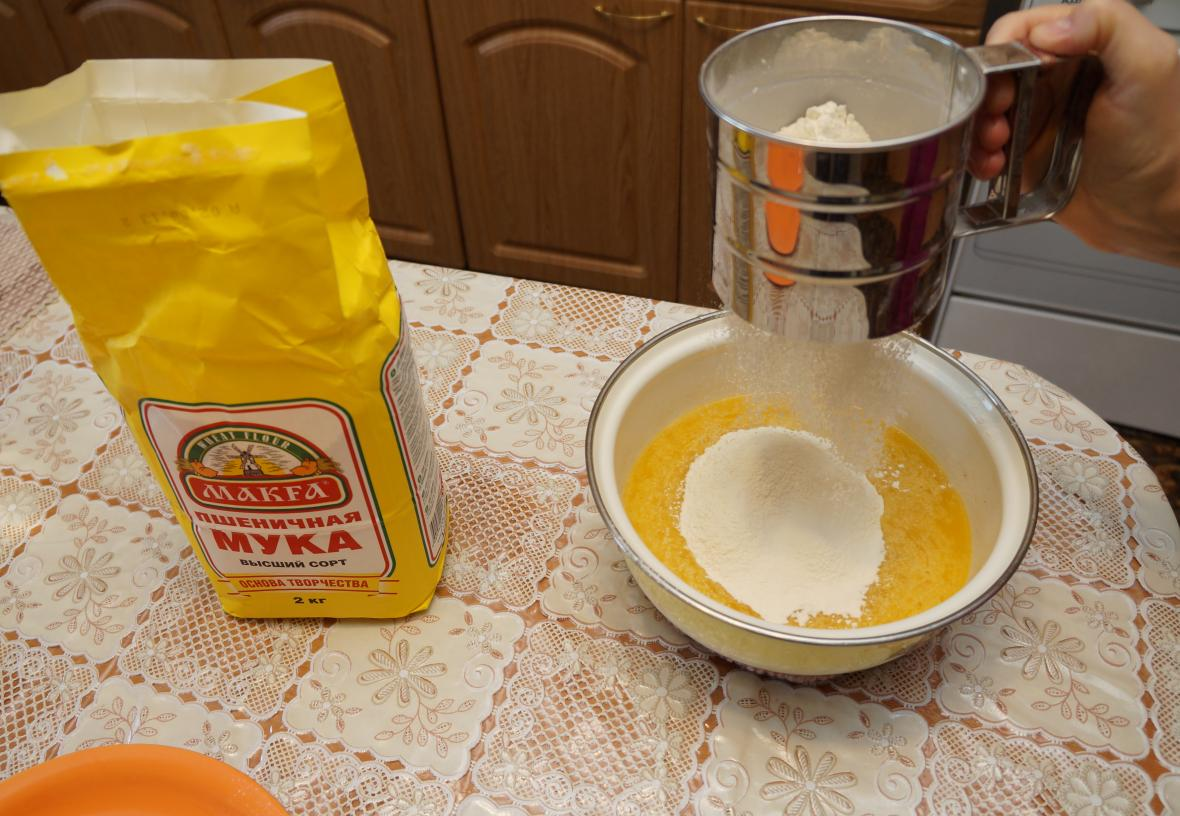
\includegraphics[height=0.65\textheight]{flour}
    \end{center}
  \end{frame}

  \begin{frame}{Тесто~--- в холодильник}
    \begin{center}
      \operation{3}{Поставить тесто на 2 часа в холодильник}

      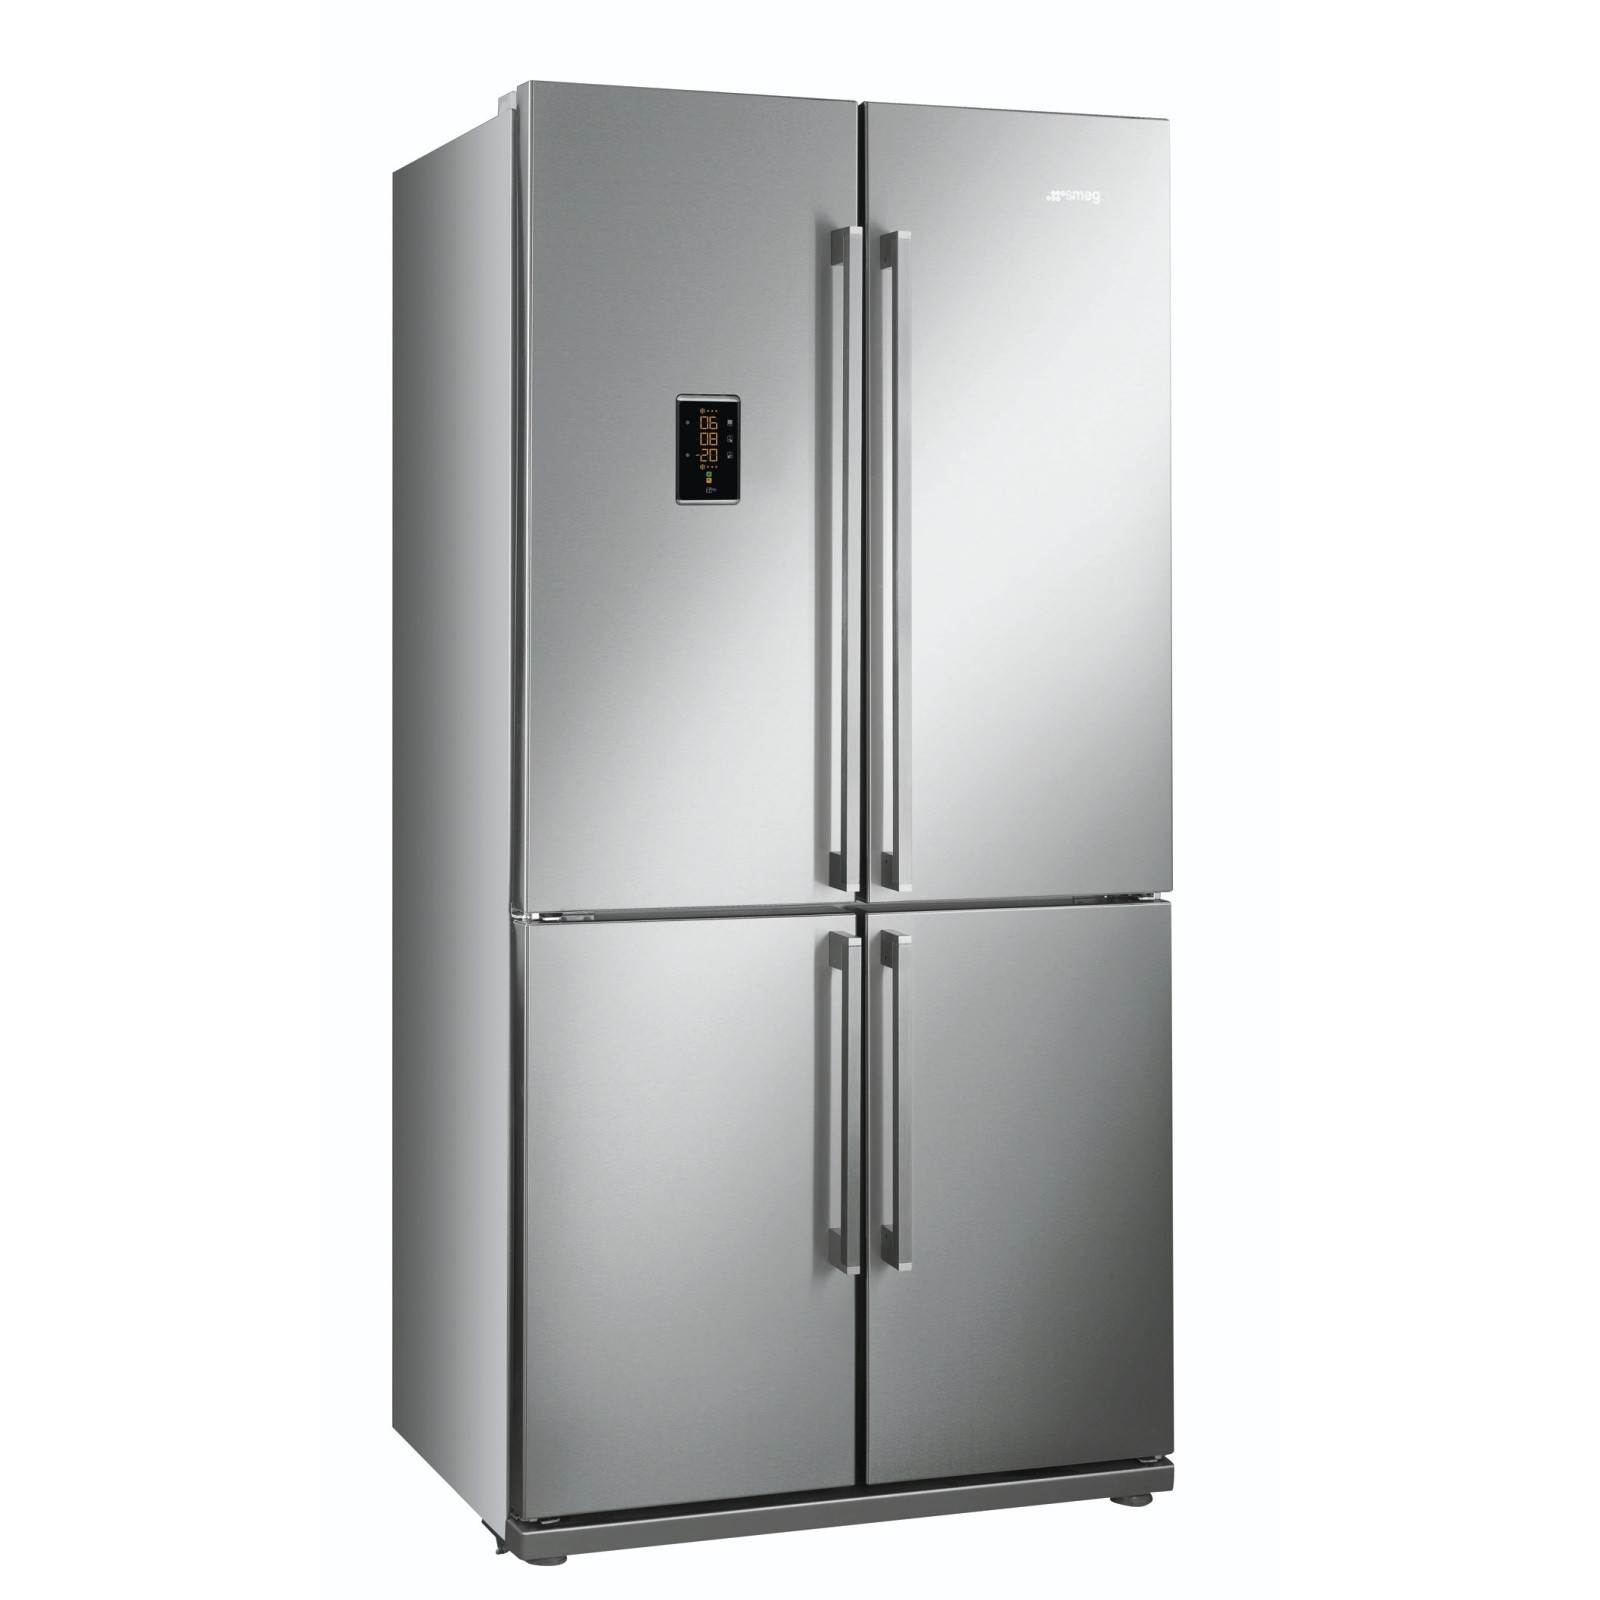
\includegraphics[height=0.7\textheight]{fridge}
    \end{center}
  \end{frame}

  \splashsection{Приготовление}

  \begin{frame}{Разделить}
    \begin{center}
      \operation{0}{Тесто \alert{(1 порция)} разделить на 8 частей}

      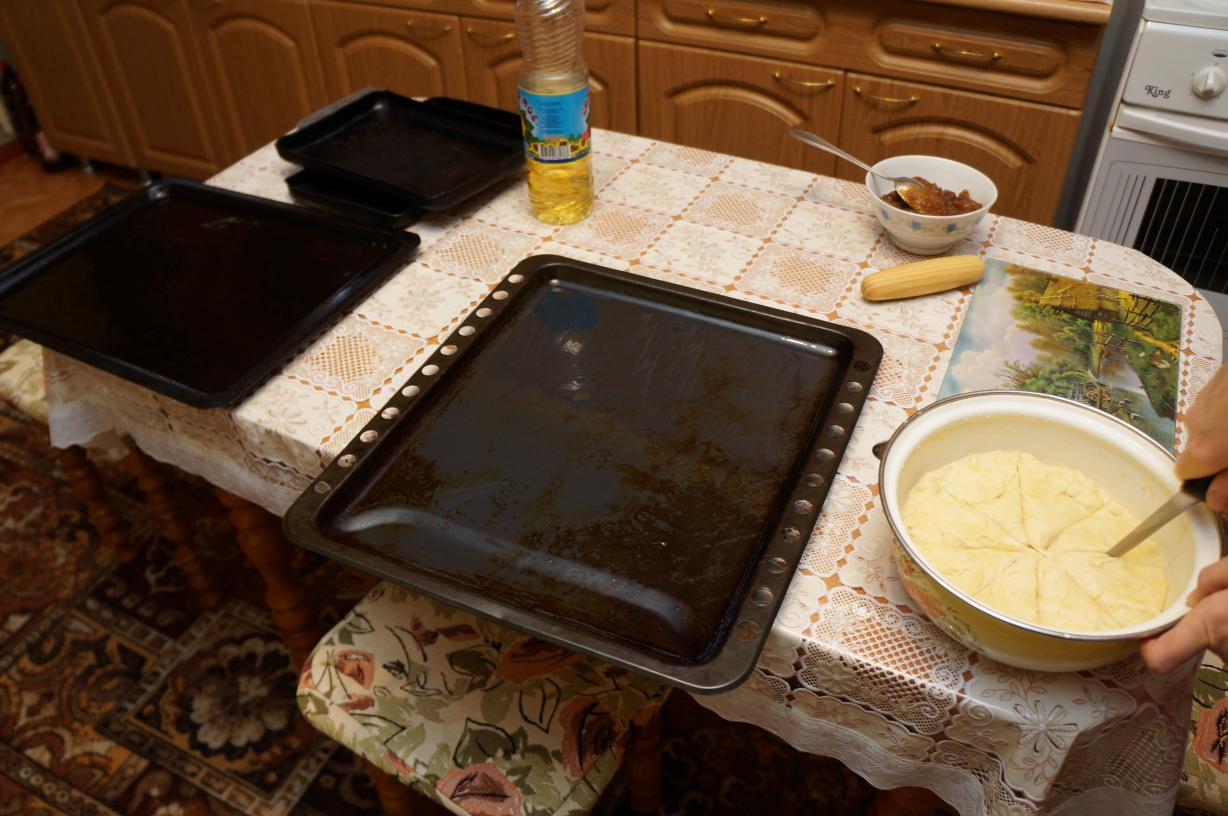
\includegraphics[height=0.7\textheight]{8parts}
    \end{center}
  \end{frame}

  \begin{frame}{Раскатать}
    \begin{center}
      \operation{1}{Раскатать тесто в прямоугольник}
      \vspace{4mm}

      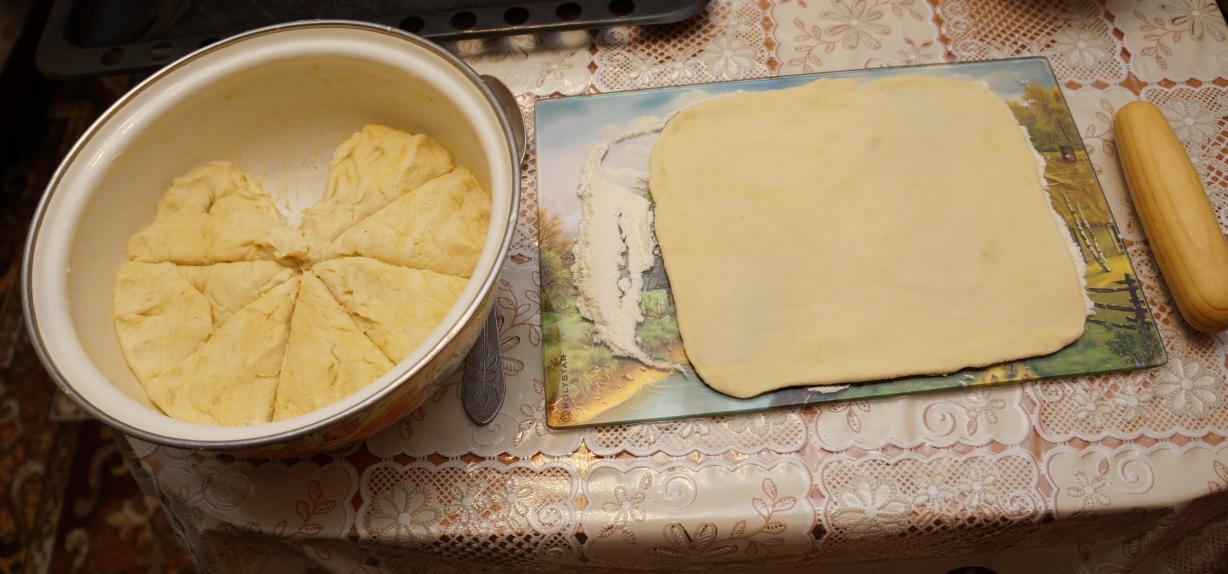
\includegraphics[width=\textwidth]{rollout}
      \vspace{5mm}
    \end{center}
  \end{frame}

  \begin{frame}{Смазать повидлом}
    \begin{center}
      \operation{2}{\alert{Половину} прямоугольника смазать повидлом}

      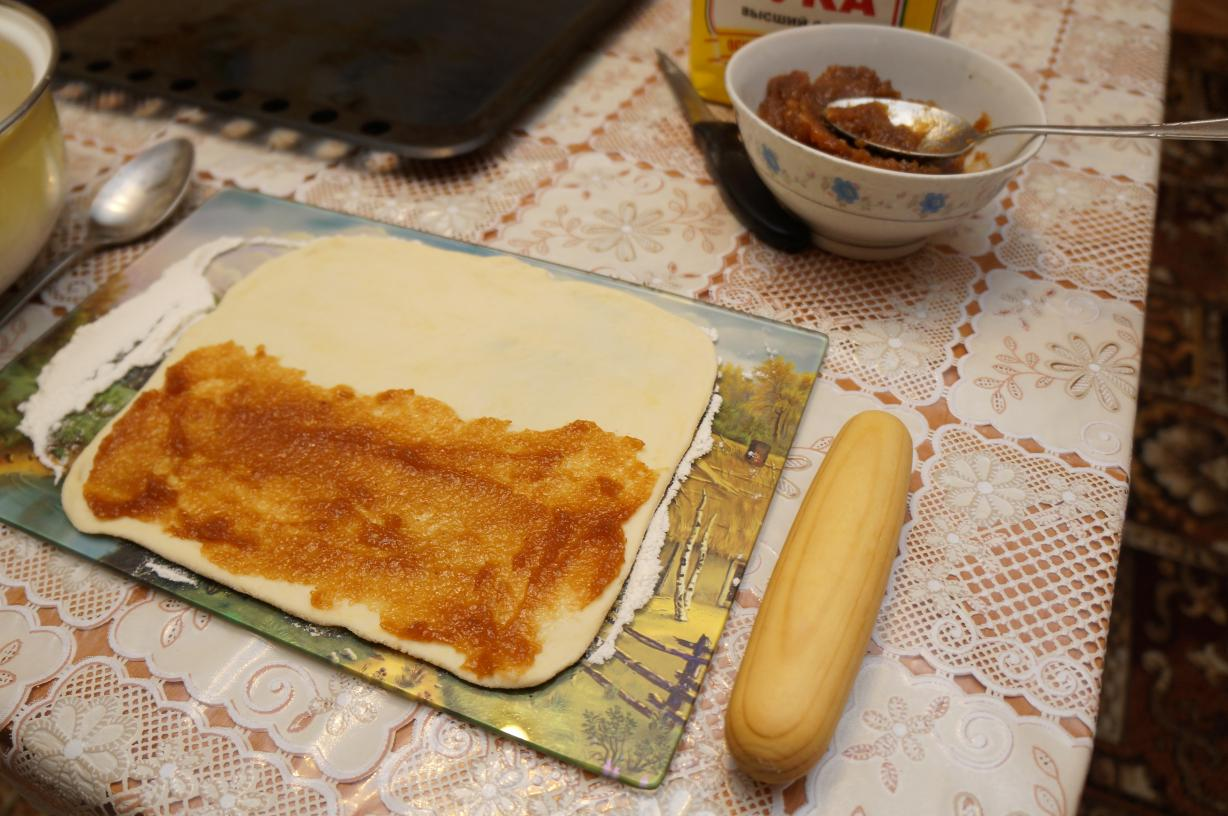
\includegraphics[height=0.7\textheight]{jam}
    \end{center}
  \end{frame}

  \begin{frame}{Смазать повидлом}
    \begin{center}
      \operation{3}{Накрыть смазанную половинку теста несмазанной\footnote{
        Если сможете купить мак, то перед переходом к следующему этапу надо
        смазать тесто взбитым яйцом и посыпать маком. Так ещё вкуснее!
      }}

      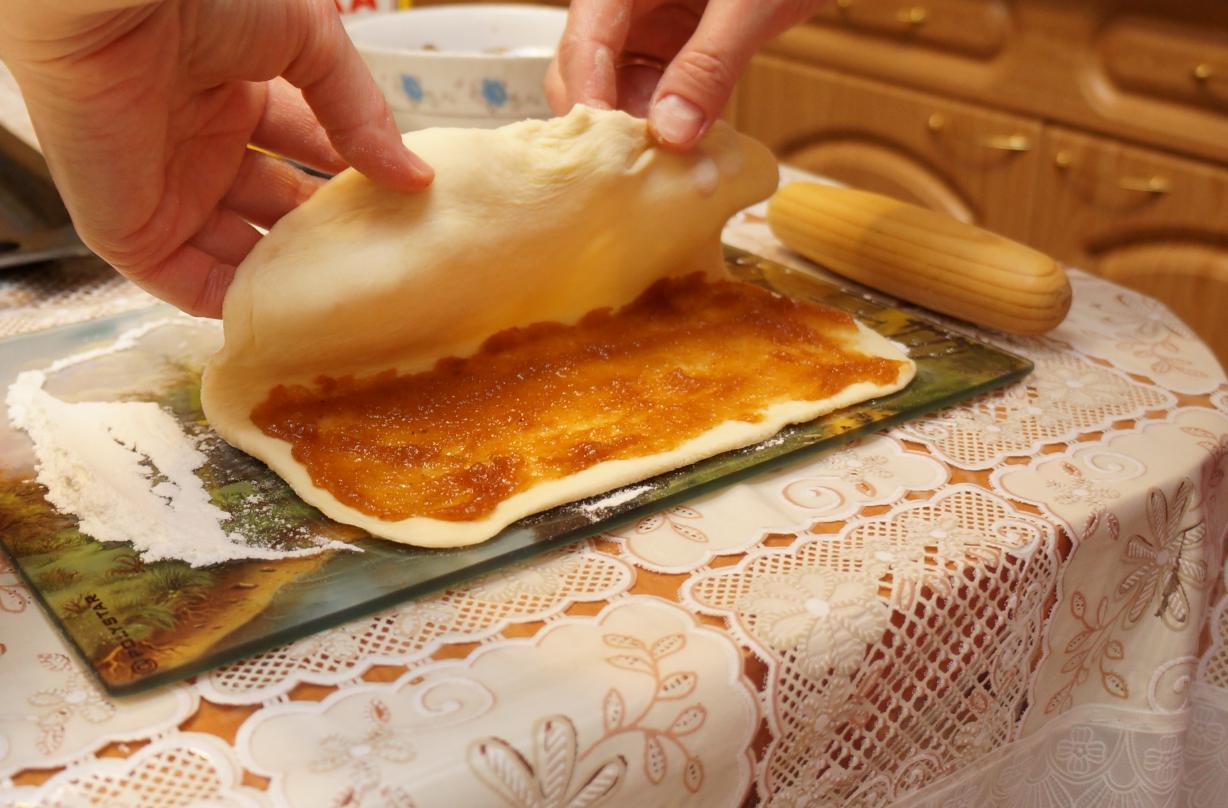
\includegraphics[height=0.62\textheight]{fold}
    \end{center}
  \end{frame}

  \begin{frame}{Нарезать}
    \begin{center}
      \operation{4}{Нарезать на полоски}

      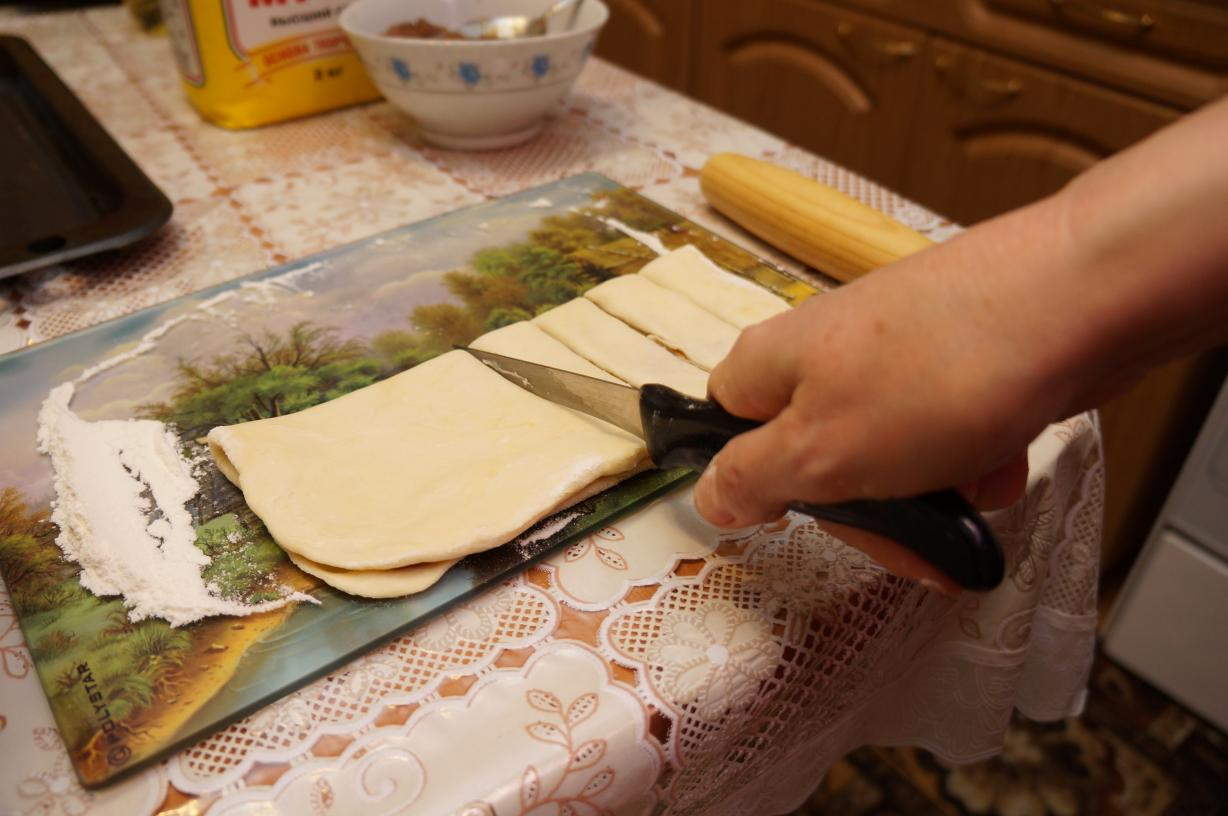
\includegraphics[height=0.7\textheight]{cut}
    \end{center}
  \end{frame}

  \begin{frame}{Выложить}
    \begin{center}
      \operation{5}{Выложить на смазанный растительным маслом противень}

      \foreach \n in {1, 2} {
        \only<\n>{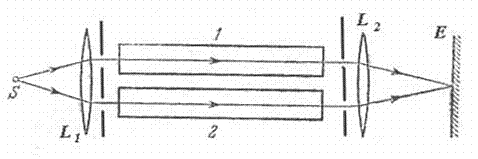
\includegraphics[height=0.7\textheight]{pan-\n}}
      }
    \end{center}
  \end{frame}

  \begin{frame}{Запечь}
    \begin{center}
      \operation{6}{Выпекать при $t = 220\text{--}250\celsius$ до
      \textcolor{Goldenrod!70!Sepia}{золотистого цвета}}

      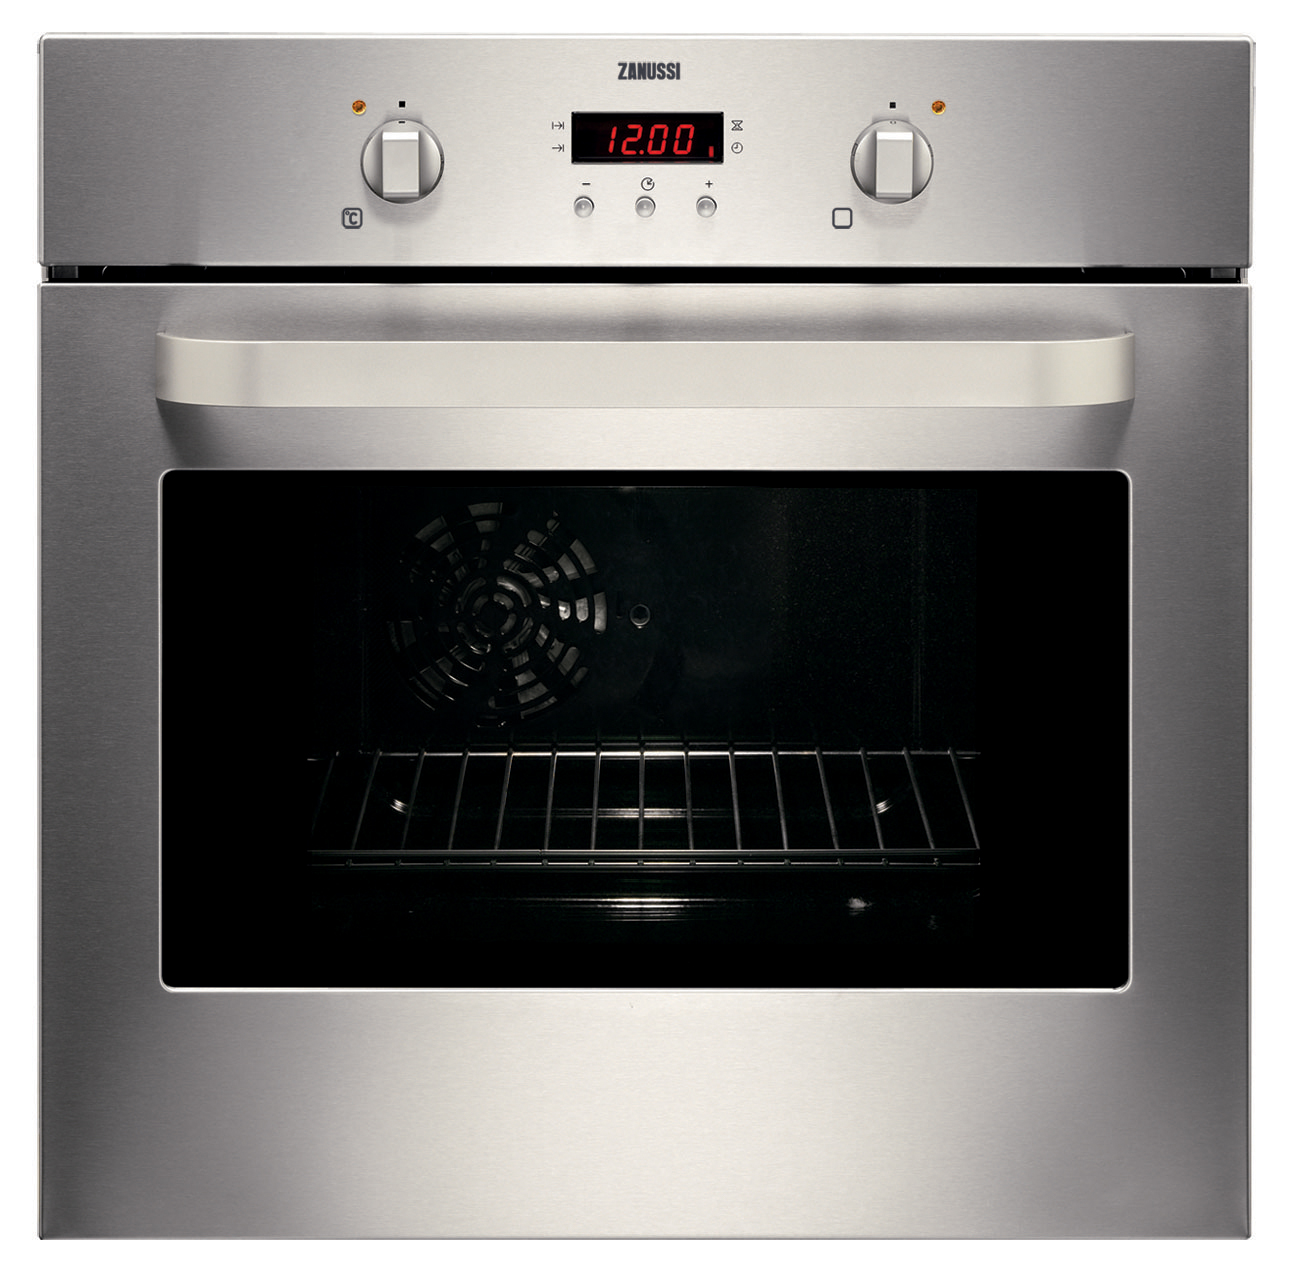
\includegraphics[height=0.7\textheight]{oven}
    \end{center}
  \end{frame}

  \begin{frame}{Приятного аппетита!}
    \begin{center}
      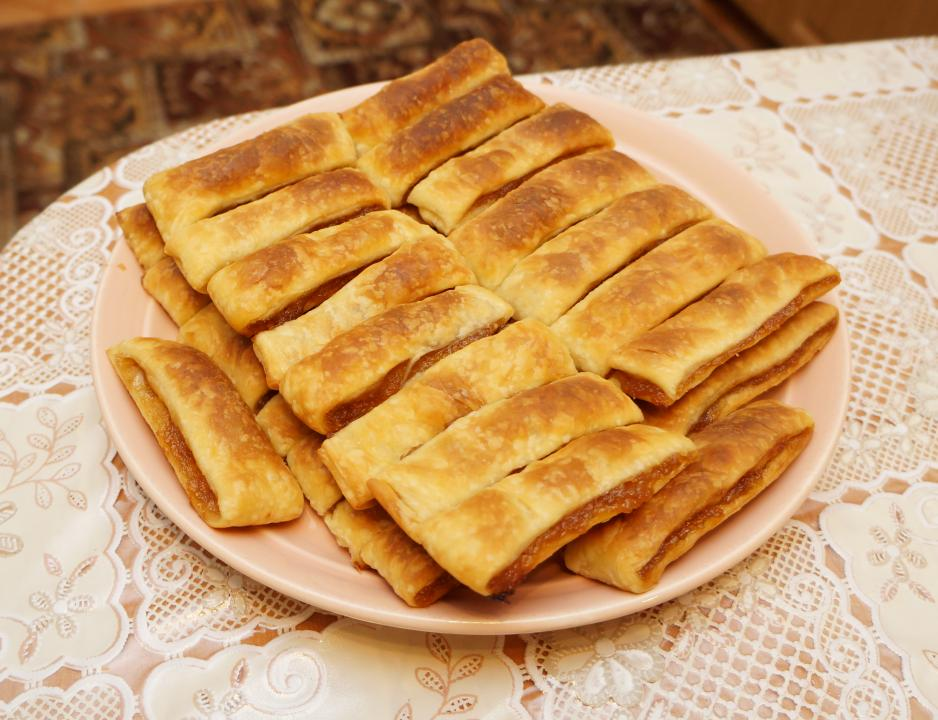
\includegraphics[height=0.82\textheight]{result}
    \end{center}
  \end{frame}

  \section{}% Заканчиваем раздел, чтобы заключение к нему не относилось
  \begin{frame}[plain]
    \begin{center}
      { \Large \LaTeX{} for life! }

      \vspace{1cm}

      Ivan Novikov\\
      \url{http://about.me/moonlighter}\\
      \href{mailto:nia.afti@gmail.com}{\nolinkurl{nia.afti@gmail.com} }
      
      \vspace{1cm}

      With Mama

    \end{center}
  \end{frame}

\end{document}

